\documentclass[aspectratio=169]{beamer}
\usepackage{will_handley}
\newcommand{\av}[2][]{\left\langle #2\right\rangle_{#1}}

% Commands
% --------
% - \arxiv{arxiv number}
% - \cols{width}{lh column}{rh column}
% -  \begin{fig(left|right)}[fractional width (e.g 0.6) ]{name of image}
%        content of other column
%    \end{fig(left|right)}

% Talk details
% ------------
\title{High dimensional nested sampling}
\date{26\textsuperscript{st} January 2023}
%Nested Sampling is an established numerical technique for optimising,
%sampling, integrating and scanning *a priori* unknown probability
%distributions. Whilst typically used in the context of traditional
%likelihood-driven Bayesian inference, it's capacity as a general sampler means
%that it is capable of exploring distributions on data [2105.13923] and joint
%spaces [1606.03757].  
%
%In this talk I will give a brief outline of the points
%of difference of nested sampling in comparison with other techniques, what it
%can uniquely offer in tackling the challenge of likelihood-free inference, and
%discuss ongoing work with collaborators in applying it in a variety of
%LFI-based approaches.

\begin{document}


\begin{frame}
    \titlepage
\end{frame}

\begin{frame}
    \frametitle{Talk structure}
    \tableofcontents
\end{frame}

\section{What is nested sampling?}
\begin{frame}
    \frametitle{What is Nested Sampling?}
    \begin{itemize}
        \item Nested sampling is a multi-purpose numerical mathematical tool.
        \item Given a (scalar) function $f$ with a vector of parameters $\theta$, it can be used for:
    \end{itemize}
    \vspace{-10pt}
    \begin{columns}[t]
        \column{0.33\textwidth}
        \begin{block}{Optimisation}
            \vspace{-5pt}
            \[\theta_\mathrm{max} = \max_\theta{f(\theta)}\]
        \end{block}
        \column{0.33\textwidth}
        \begin{block}{Sampling}
            \vspace{-5pt}
            \[\text{draw }\theta\sim f\]
        \end{block}
        \column{0.33\textwidth}
        \begin{block}{Integration}
            \vspace{-5pt}
            \[\int f(\theta) dV \]
            \vspace{-15pt}
        \end{block}
    \end{columns}
    \begin{columns}[t]
        \column{0.33\textwidth}
            \centerline{\includegraphics[width=0.8\textwidth,page=13]{figures/himmelblau}}
        \column{0.33\textwidth}
            \centerline{\includegraphics[width=0.8\textwidth,page=15]{figures/himmelblau}}
        \column{0.33\textwidth}
            \centerline{\includegraphics[width=0.8\textwidth,page=14]{figures/himmelblau}}
    \end{columns}
\end{frame}

\begin{frame}
    \frametitle{The three pillars of Bayesian inference}
    \begin{columns}[t]
        \column{0.33\textwidth}
        \begin{block}{Parameter estimation}
            What do the data tell us about the parameters of a model?

            \textit{e.g. the size or age of a $\Lambda$CDM universe}
            \[ \hspace{-10pt}\C[0]{P(\theta|D,M)} = \frac{\C[2]{P(D|\theta,M)} \C[1]{P(\theta|M)}}{\C[3]{P(D|M)}}, \] 
            \[ \C[0]{\mathcal{P}} = \frac{\C[2]{\mathcal{L}} \times\C[1]{\pi}}{\C[3]{\mathcal{Z}}}, \] 
            \[ \C[0]{\text{Posterior}} = \frac{\C[2]{\text{Likelihood}} \times\C[1]{\text{Prior}}}{\C[3]{\text{Evidence}}}. \]
        \end{block}
        \column{0.33\textwidth}
        \begin{block}{Model comparison}
            How much does the data support a particular model?

            \textit{e.g. $\Lambda$CDM vs a dynamic dark energy cosmology}
            \[ \C[4]{P(M|D)} = \frac{\C[3]{P(D|M)} \C[5]{P(M)}}{\C[7]{P(D)}}, \] \[ \frac{\C[3]{\mathcal{Z}_\mathcal{M}} \C[5]{\Pi_\mathcal{M}}}{\C[7]{\sum_m Z_m \Pi_m}}, \] \[ \C[4]{\text{Posterior}} = \frac{\C[3]{\text{Evidence}} \times\C[5]{\text{Prior}}}{\C[7]{\text{Normalisation}}}.\]
        \end{block}
        \column{0.33\textwidth}
        \begin{block}{Tension quantification}
            Do different datasets make consistent predictions from the same model? 

            \textit{e.g. CMB vs Type IA supernovae data}
            \[ \mathcal{R} = \frac{\C[3]{\mathcal{Z}}_{AB}}{\C[3]{\mathcal{Z}}_A\C[3]{\mathcal{Z}}_\mathcal{B}}, \] 
            \[
                \begin{aligned} \log\mathcal{S} = \av[{\C[0]{\mathcal{P}}_{AB}}]{\C[2]{\log\mathcal{L}}_{AB}}&\\
                    -\av[{\C[0]{\mathcal{P}}_{A}}]{\C[2]{\log\mathcal{L}}_{A}}&\\
                    -\av[{\C[0]{\mathcal{P}}_{B}}]{\C[2]{\log\mathcal{L}}_{B}}&
                \end{aligned}
            \]
        \end{block}
    \end{columns}
\end{frame}


\begin{frame}
    \frametitle{Why do sampling?}
    \begin{columns}
        \column{0.5\textwidth}
        \begin{itemize}
            \item The cornerstone of numerical Bayesian inference is working with \textbf{samples}.
            \item Generate a set of representative parameters drawn in proportion to the posterior $\theta\sim\C[0]{\mathcal{P}}$.
            \item The magic of marginalisation $\Rightarrow$ perform usual analysis on each sample in turn.
            \item The golden rule is \C[3]{stay in samples} until the last moment before computing summary statistics/triangle plots because \[\boxed{f(\:\av{X}\:)\ne \av{\:f(X)\:}}\]
            \item Generally need $\sim\mathcal{O}(12)$ independent samples to compute a value and error bar.
        \end{itemize}
        \column{0.5\textwidth}
        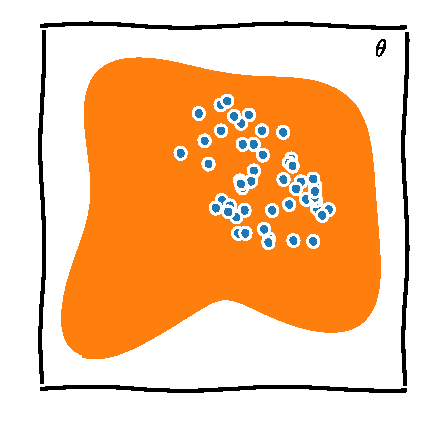
\includegraphics{figures/samples.pdf}
    \end{columns}
\end{frame}

\begin{frame}
    \begin{columns}
        \column{0.5\textwidth}
        \begin{block}{\textbf{MCMC}}
            \includegraphics<1>[width=\textwidth,page=16]{figures/himmelblau}%
            \includegraphics<2>[width=\textwidth,page=17]{figures/himmelblau}%
            \includegraphics<3>[width=\textwidth,page=18]{figures/himmelblau}%
            \includegraphics<4>[width=\textwidth,page=19]{figures/himmelblau}%
            \includegraphics<5>[width=\textwidth,page=20]{figures/himmelblau}%
            \includegraphics<6-15>[width=\textwidth,page=21]{figures/himmelblau}%
            \begin{itemize}
                \item<16> Single ``walker''
                \item<16> Explores posterior
                \item<16> Fast, if proposal matrix is tuned
                \item<16> Parameter estimation, suspiciousness calculation
                \item<16> Channel capacity optimised for generating posterior samples
            \end{itemize}
        \end{block}
        \centerline{\includegraphics<16>[width=0.5\textwidth,page=19]{figures/himmelblau}}
        \column{0.5\textwidth}
        \begin{block}<7->{\textbf{Nested sampling}}
            \includegraphics<7|handout:0>[width=\textwidth,page=1]{figures/himmelblau}%
            \includegraphics<8|handout:0>[width=\textwidth,page=2]{figures/himmelblau}%
            \includegraphics<9|handout:0>[width=\textwidth,page=3]{figures/himmelblau}%
            \includegraphics<10          >[width=\textwidth,page=4]{figures/himmelblau}%
            \includegraphics<11|handout:0>[width=\textwidth,page=5]{figures/himmelblau}%
            \includegraphics<12|handout:0>[width=\textwidth,page=6]{figures/himmelblau}%
            \includegraphics<13|handout:0>[width=\textwidth,page=7]{figures/himmelblau}%
            \includegraphics<14|handout:0>[width=\textwidth,page=8]{figures/himmelblau}%
            \includegraphics<15|handout:0>[width=\textwidth,page=15]{figures/himmelblau}%
            \begin{itemize}
                \item<16> Ensemble of ``live points''
                \item<16> Scans from prior to peak of likelihood
                \item<16> Slower, no tuning required
                \item<16> Parameter estimation, model comparison, tension quantification
                \item<16> Channel capacity optimised for computing partition function
            \end{itemize}
        \centerline{\includegraphics<16>[width=0.5\textwidth,page=4]{figures/himmelblau}} \end{block}
    \end{columns}
\end{frame}

\begin{frame}
    \frametitle{Nested sampling}
    \begin{columns}
        \column{0.6\textwidth}
        \begin{itemize}
            \item Sequentially update a set $S$ of $n$ samples:
                \begin{itemize}
                    \item[$S_0$:]  Generate $n$ samples uniformly over the space (from the prior $\pi$). 

                    \item[$S_{i+1}$:] Delete the lowest likelihood sample in $S_{i}$, and replace it with a new uniform sample with higher likelihood.
                \end{itemize}
            \item Requires one to be able to sample uniformly within a region, subject to a {\em hard likelihood constraint}:
                \[\{\theta\sim \pi : \mathcal{L}(\theta)>\mathcal{L}_*. \}\]
            \item This procedure optimises (multimodally), and can calculate the \C[3]{evidence} \& \C[0]{posterior} weights.
            \item The evolving ensemble of live points allows algorithms to perform self-tuning and mode clustering.
        \end{itemize}
        \column{0.4\textwidth}
        \includegraphics[width=\textwidth,page=8]{figures/himmelblau}%
    \end{columns}
\end{frame}

\begin{frame}
    \frametitle{Probabalistic volume estimation}
    \begin{columns}
        \column{0.5\textwidth}
        \begin{itemize}
            \item Key idea in NS: estimating volumes probabilistically
        \end{itemize}
        \[
            \frac{\C[1]{V_\mathrm{after}}}{\C[0]{V_\mathrm{before}}} 
            \approx \frac{\C[1]{n_\mathrm{in}}}{\C[0]{n_\mathrm{out}}+\C[1]{n_\mathrm{in}}}
        \]
        \column{0.5\textwidth}
        \includegraphics<1>[width=\textwidth]{figures/compression_1}%
        \includegraphics<2->[width=\textwidth]{figures/compression_2}%
    \end{columns}
\end{frame}

\begin{frame}
    \frametitle{Dead points: posteriors \& evidences}
    \begin{columns}
        \column{0.6\textwidth}
        \begin{itemize}
            \item At the end, one is left with a set of discarded points.
            \item These may be weighted to form weighted posterior samples using $w_i = \mathcal{L}_i \Delta X_i$.
            \item They can also be used to calculate the normalisation $\mathcal{Z} = \sum \mathcal{L}_i \Delta X_i$, or more generally $\sum_i f(\mathcal{L}_i) \Delta X_i$.
                \begin{itemize}
                    \item Nested sampling probabilistically estimates the volume of the parameter space
                        \[X_i \approx {\left(\frac{n}{n+1}\right)} X_{i-1} \quad\Rightarrow\quad
                        X_i \approx {\left(\frac{n}{n+1}\right)}^i \approx e^{-i/n}, \]
                    \item Nested sampling thus estimates the density of states,
                    \item it is therefore a partition function calculator
                        $Z(\beta) = \sum_i \mathcal{L}_i^\beta \Delta X_i$.
                \end{itemize}
        \end{itemize}

        \column{0.4\textwidth}

        \includegraphics<1|handout:0>[width=\textwidth,page=14]{figures/himmelblau}%
        \includegraphics<2          >[width=\textwidth,page=15]{figures/himmelblau}%

    \end{columns}

\end{frame}

\begin{frame}
  \frametitle{Sampling from a hard likelihood constraint} 
  
  \begin{quote}
    ``It is not the purpose of this introductory paper to develop the technology of navigation within such a volume. We merely note that exploring a hard-edged likelihood-constrained domain should prove to be neither more nor less demanding than exploring a likelihood-weighted space.''
    
   {\hfill --- John Skilling}
  \end{quote}

  \begin{itemize}
      
    \item A large fraction of the work in NS to date has been in attempting to implement a hard-edged sampler in the NS meta-algorithm $\{\theta\sim \pi : \mathcal{L}(\theta)>\mathcal{L}_* \}$.
    \item \url{https://projecteuclid.org/euclid.ba/1340370944}.
    \item There has also been much work beyond this (focus of this talk).
  \end{itemize}
 
\end{frame}


\begin{frame}
    \frametitle{Implementations of Nested Sampling}
    \begin{columns}[t]
        \column{0.3\textwidth}
        \texttt{MultiNest}~\arxiv{0809.3437}
        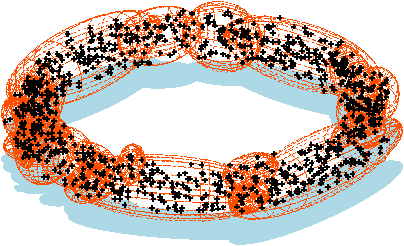
\includegraphics[width=\textwidth]{figures/multinest}
        \texttt{UltraNest}~\arxiv{2101.09604}
        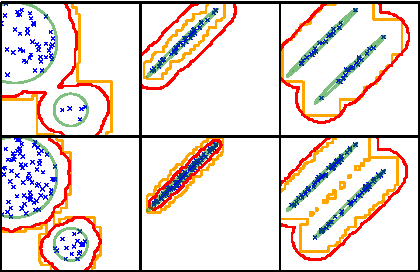
\includegraphics[width=\textwidth]{figures/radfriends}
        \column{0.4\textwidth}
        \texttt{PolyChord}~\arxiv{1506.00171}
        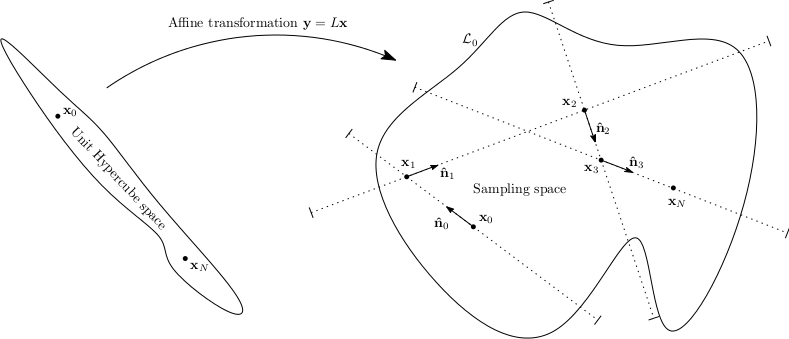
\includegraphics[width=\textwidth]{figures/polychord}
        \vfill
        \texttt{NeuralNest}~\arxiv{1903.10860}
        \begin{columns}
            \column{0.5\textwidth}
            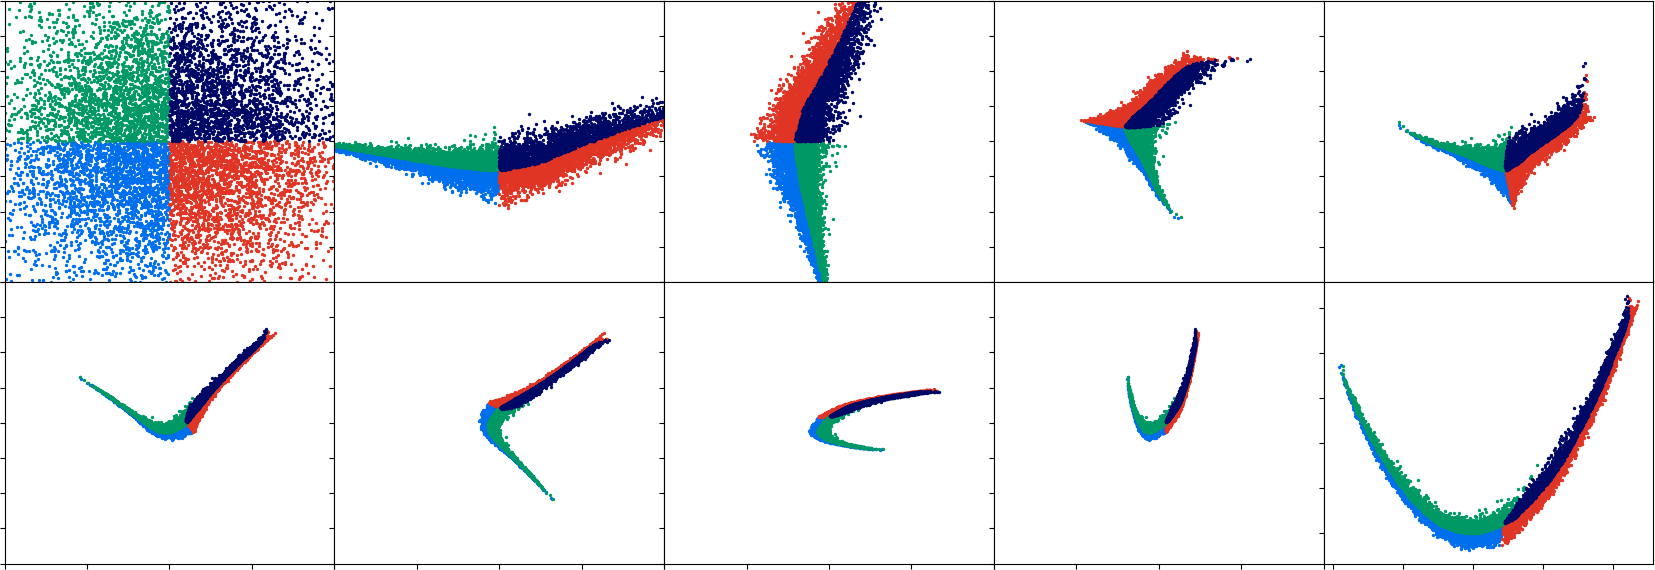
\includegraphics[width=\textwidth]{figures/rosenbrock_flow.png}
            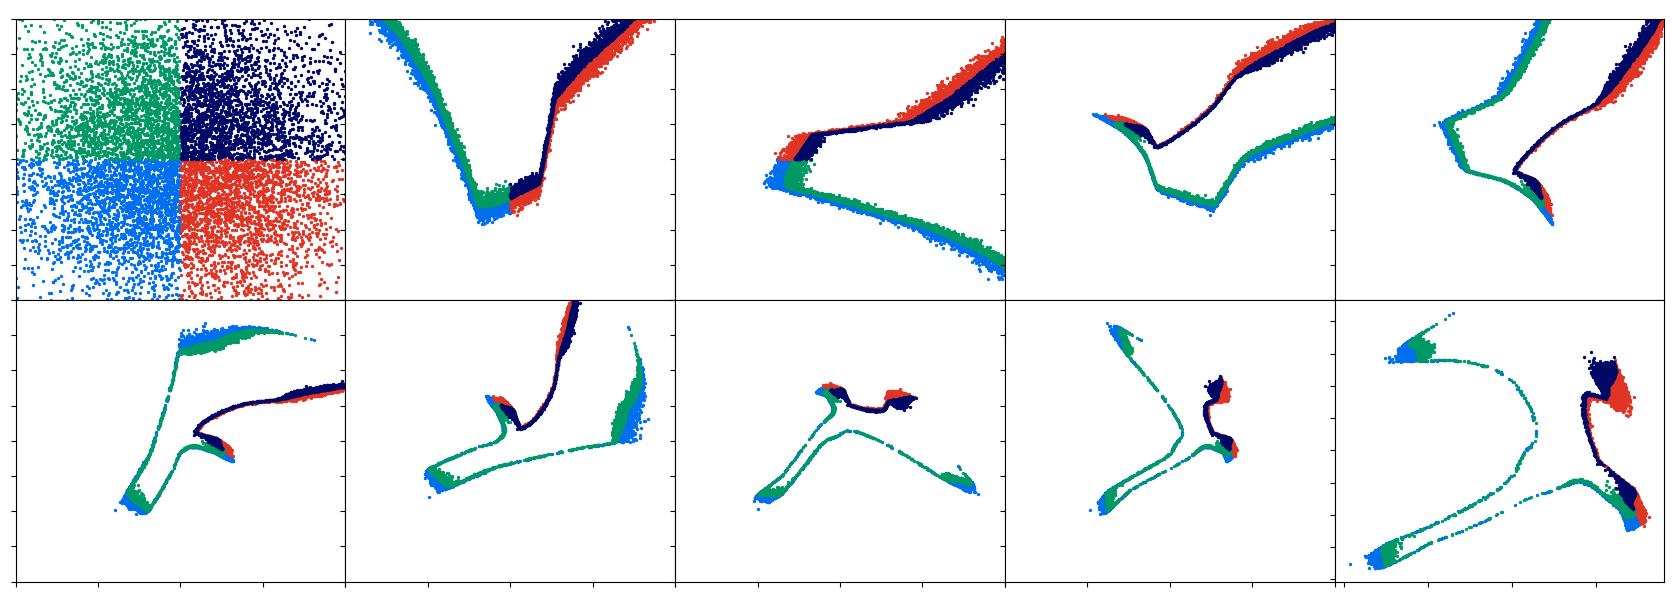
\includegraphics[width=\textwidth]{figures/himmelblau_flow.png}
            \column{0.5\textwidth}
            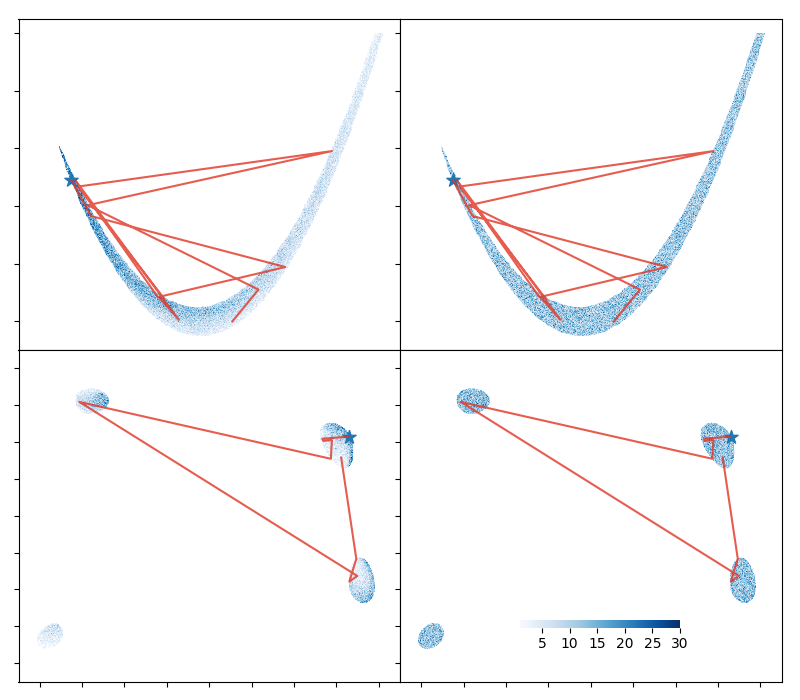
\includegraphics[width=\textwidth]{figures/chains.png}
        \end{columns}
        \texttt{dynesty}~\arxiv{1904.02180}
        \vfill
        \column{0.3\textwidth}
        \texttt{DNest}~\arxiv{1606.03757}
        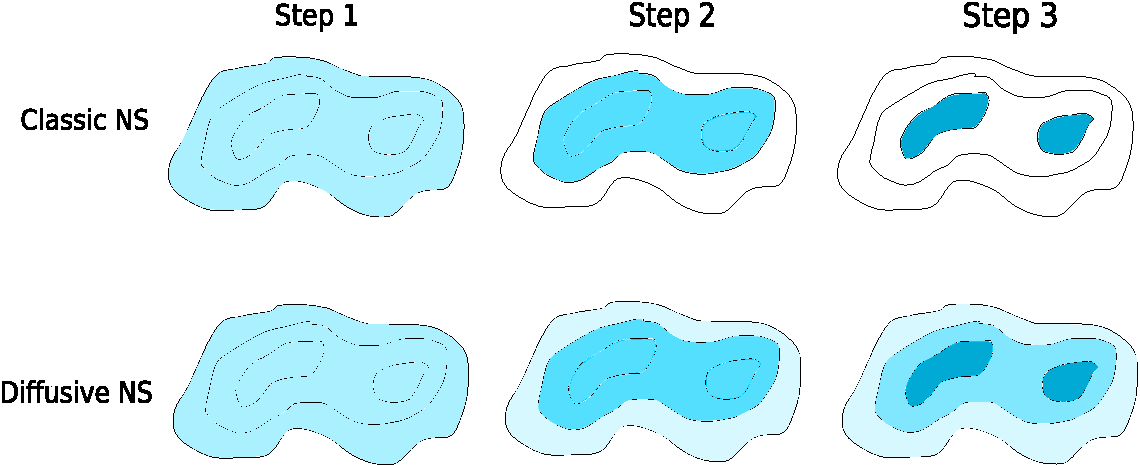
\includegraphics[width=\textwidth]{figures/dnest}
        \texttt{ProxNest}~\arxiv{2106.03646}
        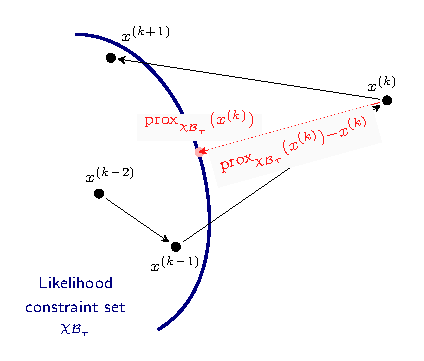
\includegraphics[width=\textwidth]{figures/proxnest_diagram}
        \vfill
    \end{columns}
\end{frame}

\begin{frame}
    \frametitle{Types of nested sampler}
    \begin{itemize}
        \item Broadly, most nested samplers can be split into how they create new live points.
        \item i.e. how they sample from the hard likelihood constraint $\{\theta\sim \pi : \mathcal{L}(\theta)>\mathcal{L}_* \}$.
    \end{itemize}
    \vspace{-10pt}
    \begin{columns}[t]
        \column{0.5\textwidth}
        \begin{block}{Rejection samplers}
            \begin{itemize}
                \item e.g. \texttt{MultiNest}, \texttt{UltraNest}.
                \item Constructs bounding region and draws many invalid points until one is found within $L_*$.
                \item Efficient in low dimensions, exponentially inefficient $\sim\mathcal{O}(e^{d/d_0})$ in high  $d>d_0\sim10$.
            \end{itemize}
        \end{block}
        \column{0.5\textwidth}
        \begin{block}{Chain-based samplers}
            \begin{itemize}
                \item e.g. \texttt{PolyChord}, \texttt{ProxNest}.
                \item Run Markov chain starting at a live point, generating many valid (correlated) points.
                \item Linear $\sim\mathcal{O}(d)$ penalty in decorrelating new live point from the original seed point.
            \end{itemize}
        \end{block}
    \end{columns}
    \vspace{15pt}
    \begin{itemize}
        \item Nested samplers usually come with:
            \begin{itemize}
                \item \emph{resolution} parameter $n_\mathrm{live}$ (which improve results as $\sim\mathcal{O}(n_\mathrm{live}^{-1/2})$.
                    \item set of \emph{reliability} parameters~\arxiv{2101.04525}, which don't improve results if set arbitrarily high, but introduce systematic errors if set too low.
                    \item e.g. \texttt{Multinest} efficiency \texttt{eff} or \texttt{PolyChord} chain length $n_\mathrm{repeats}$.
            \end{itemize}
    \end{itemize}
\end{frame}

\begin{frame}
    \frametitle{How does Nested Sampling compare to other approaches?}
    \begin{columns}
        \column{0.7\textwidth}
    \begin{itemize}
        \item In all cases:
            \begin{itemize}
                \item[$+$] NS can handle multimodal functions
                \item[$+$] NS computes evidences, partition functions and integrals
                \item[$+$] NS is self-tuning/black-box
            \end{itemize}
    \end{itemize}
        \column{0.3\textwidth}
        Modern Nested Sampling algorithms can do this in $\sim\mathcal{O}(100s)$ dimensions
    \end{columns}
    \begin{columns}[t]
        \column{0.33\textwidth}
        \begin{block}{Optimisation}
        \begin{itemize}
            \item Gradient descent
                \begin{itemize}
                    \item[$+$] NS does not require gradients
                \end{itemize}
            \item Genetic algorithms
                \begin{itemize}
                    \item[$+$] NS discarded points have statistical meaning
                \end{itemize}
        \end{itemize}
        \end{block}
        \column{0.33\textwidth}
        \begin{block}{Sampling}
        \begin{itemize}
            \item Metropolis-Hastings?
                \begin{itemize}
                    \item[$-$] Very little beats a well-tuned, customised MH
                    \item[$+$] NS is self tuning
                \end{itemize}
        \item Hamiltonian Monte Carlo?
        \begin{itemize}
            \item[$-$] In millions of dimensions, HMC is king
            \item[$+$] NS does not require gradients
        \end{itemize}
        \end{itemize}
            \end{block}
        \column{0.33\textwidth}
        \begin{block}{Integration}
            \begin{itemize}
                \item Thermodynamic integration
                    \begin{itemize}
                        \item[$+$] protective against phase trasitions
                        \item[$+$] No annealing schedule tuning 
                    \end{itemize}
                \item Sequential Monte Carlo
                    \begin{itemize}
                        \item[$-$] Some people (SMC experts) classify NS as a kind of SMC
                        \item[$+$] NS is athermal
                    \end{itemize}
            \end{itemize}
    \end{block}
    \end{columns}
\end{frame}



\begin{frame}
    \frametitle{Nested Sampling with Likelihood Free Inference}
    \begin{columns}
        \column{0.5\textwidth}
        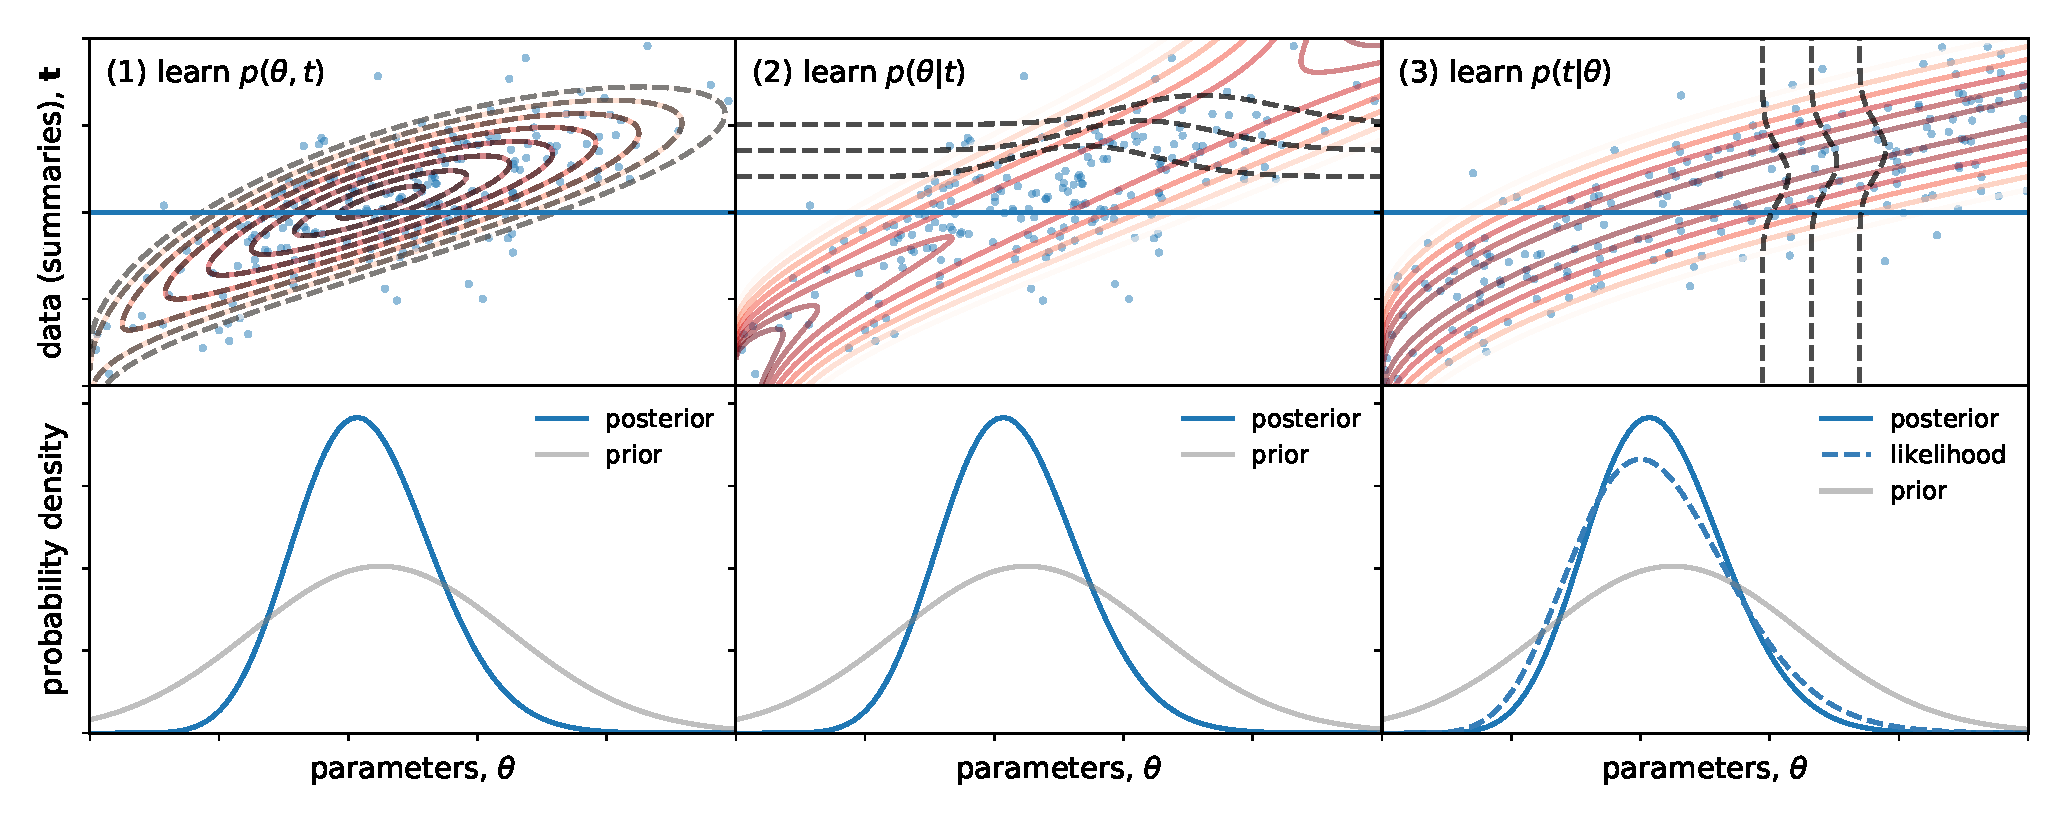
\includegraphics[width=\textwidth]{figures/three_ways_II.pdf}

        \hfill Alsing \textit{et al.}~\arxiv{1903.00007}
    \begin{itemize}
        \item In density estimation likelihood free inference, the output is to learn one/all of:
            \begin{description}
                \item[Likelihood] $P(D|\theta)$
                \item[Posterior] $P(\theta|D)$ 
                \item[Joint] $P(D,\theta)$
            \end{description}
        \item In the first instance, nested sampling can be used to scan these learnt functions
    \end{itemize}
        \column{0.5\textwidth}
    \begin{itemize}
        \item Data are compressed, so joint space $(D,\theta)$ is navigable by off-the-shelf codes. 
            \begin{itemize}
                \item Sanity checking the solution
                \item Computing evidences/Kullback Liebler divergences from likelihoods
            \end{itemize}
        \item Its self-tuning capacity and ability to handle multi-modal distributions can be very useful for diagnosing incompletely learnt functions
        \item Emulated likelihoods (e.g. normalising flows) are generally fast, so can deploy more likelihood hungry techniques like NS.
        \item As Pablo Lemos \& David Yallup will discuss, in principle can use it to train emulators by marginalisation rather than maximisation.
    \end{itemize}
    \end{columns}
\end{frame}

\begin{frame}
    \frametitle{Nested Sampling for Approximate Bayesian Computation/SBI}
    \begin{columns}
        \column{0.5\textwidth}
        \begin{itemize}
            \item Assume one has a generative model capable of turning parameters into mock data $D(\theta)$
            \item Given infinite computing power, ABC works by selecting $\{\theta : D(\theta)=D_\mathrm{observed}\}$
            \item These are samples from the posterior, without using a likelihood.
            \item In practice $D=D_\mathrm{obs}$ becomes $D\approx D_\mathrm{obs}$
            \item i.e. $|D-D_\mathrm{obs}|<\varepsilon$, or more generally $\boxed{\rho(D,D_\mathrm{obs})<\varepsilon}$, where $\rho$ is some suitably chosen objective function
            \item Main challenges are 
                \begin{enumerate}
                    \item Choice of $\rho$/summary stats
                    \item Choice of $\varepsilon$ schedule
                    \item Rejection sampling
                \end{enumerate}
        \end{itemize}
        \column{0.5\textwidth}
        \begin{itemize}
            \item Nested sampling fits this well: In principle, can just change the usual hard likelihood constraints $\{\theta\sim\pi : \mathcal{L}(\theta)>\mathcal{L}_*\}$ to
                \[\{\theta~\sim\pi : \rho(D(\theta),D_\mathrm{obs})<\varepsilon\}\]
            (Brewer \& Foreman-Mackey~\arxiv{1606.03757})
            \item Ongoing work with Andrew Fowlie \& Sebastian Hoof
                \begin{itemize}
                    \item How to deal with nondeterminism 
                    \item How to interpret $\rho$ as a ``likelihood''
                    \item How to interpret the evidence $\mathcal{Z}$
                \end{itemize}
        \end{itemize}
    \end{columns}
\end{frame}

\begin{frame}
    \frametitle{Nested sampling as an optimiser}
    <++>
\end{frame}

%\begin{frame}
%    \frametitle{<+Title+>}
%    <+Content+>
%\end{frame}


\begin{frame}
    \frametitle{Nested Sampling: a user's guide}
    \begin{enumerate}
        \item Nested sampling is a likelihood scanner, rather than posterior explorer.
            \begin{itemize}
                \item This means typically most of its time is spent on burn-in rather than posterior sampling
                \item Changing the stopping criterion from $10^{-3}$ to $0.5$ does little to speed up the run, but can make results very unreliable
            \end{itemize}
        \item The number of live points $n_\mathrm{live}$ is a resolution parameter.
            \begin{itemize}
                \item Run time is linear in $n_\mathrm{live}$, posterior and evidence accuracy goes as $\frac{1}{\sqrt{n_\mathrm{live}}}$.
                \item Set low for exploratory runs $\sim\mathcal{O}(10)$ and increased to $\sim\mathcal{O}(1000)$ for production standard.
                \item Extreme MPI parallelisation means walltime can be made constant.
            \end{itemize}
        \item Most algorithms come with additional reliability parameter(s).
            \begin{itemize}
                \item e.g. \texttt{MultiNest}: $\text{eff}$, \texttt{PolyChord}: $n_\mathrm{repeats}$
                \item These are parameters which have no gain if set too conservatively, but increase the reliability
                \item Check that results do not degrade if you reduce them from defaults, otherwise increase.
            \end{itemize}
    \end{enumerate}
\end{frame}

\begin{frame}
    \frametitle{A note on dynesty}
\end{frame}

\begin{frame}
    \frametitle{Key tools for Nested Sampling}
    \begin{description}[\& \texttt{UltraNest}]
        \item[\texttt{anesthetic}] Nested sampling post processing \arxiv{1905.04768}\\
        \item[\texttt{insertion}] cross-checks using order statistics \arxiv{2006.03371}
            \hspace{5pt}\url{github.com/williamjameshandley/anesthetic}
        \item[\texttt{nestcheck}] cross-checks using unthreaded runs \arxiv{1804.06406}\\
            \hspace{5pt}\url{github.com/ejhigson/nestcheck}
        \item[\texttt{MultiNest}] Ellipsoidal rejection sampling \arxiv{0809.3437}\\
            \hspace{5pt}\url{github.com/farhanferoz/MultiNest}
        \item[\texttt{PolyChord}] Python/C++/Fortran state of the art \arxiv{1506.00171}\\
            \hspace{5pt}\url{github.com/PolyChord/PolyChordLite} 
        \item[\texttt{dynesty}] Python re-implementation of several codes \arxiv{1904.02180}\\
            \hspace{5pt}\url{github.com/joshspeagle/dynesty}
        \item[\& \texttt{UltraNest}] \hspace{5pt}\url{github.com/JohannesBuchner/UltraNest}
            \arxiv{2101.09604}
        \item[\texttt{SuperNest}] Accelerated nested sampling with prior repartitioning \arxiv{2212.01760}
    \end{description}
\end{frame}


\appendix



\begin{frame}
    \frametitle{Occam's Razor~\arxiv{2102.11511}}
    \begin{itemize}
        \item Bayesian inference quantifies Occam's Razor:
            \begin{itemize}
                \item \textit{``Entities are not to be multiplied without necessity''} \hfill --- William of Occam
                \item \textit{``Everything should be kept as simple as possible, but not simpler''} \hfill --- ``Albert Einstein''
            \end{itemize}
        %\item Consider the Evidence $\C[3]{\mathcal{Z}\equiv P(D|M)}$: 
        %    \begin{description}[Parameter estimation]
        %        \item [Parameter estimation] normalisation constant
        %        \item [Model comparison] critical update factor for \C[5]{model prior} to \C[4]{model posterior}
        %    \end{description}
        \item Properties of the evidence: rearrange Bayes' theorem for parameter estimation
            \[\C[0]{\mathcal{P}(\theta)} = \frac{\C[2]{\mathcal{L}(\theta)} \C[1]{\pi(\theta)}}{\C[3]{\mathcal{Z}}} \qquad\Rightarrow\qquad \C[3]{\log \mathcal{Z}} = \C[2]{\log\mathcal{L}(\theta)} - \log \frac{\C[0]{\mathcal{P}(\theta)}}{\C[1]{\pi(\theta)}} \]  
        \item Evidence is composed of a ``goodness of fit'' term  and ``Occam Penalty''
    \end{itemize}
    \begin{columns}[t]
        \column{0.5\textwidth}
    \begin{itemize}
        \item RHS true for all $\theta$. Take max likelihood value $\theta_*$:
            \[
                \log \mathcal{Z} = -\chi_\mathrm{min}^2 - \text{Mackay penalty}
            \]
    \end{itemize}
        \column{0.5\textwidth}
    \begin{itemize}
        \item Be more Bayesian and take posterior average to get the ``Occam's razor equation''
            \[
                \boxed{
                    \log \mathcal{Z} = \av[\mathcal{P}]{\log\mathcal{L}} - \mathcal{D}_\mathrm{KL}
            }
            \]
    \end{itemize}
    \end{columns}
    \vfill
    \begin{itemize}
        \item Natural regularisation which penalises models with too many parameters.
    \end{itemize}
\end{frame}

\begin{frame}
    \frametitle{Kullback Liebler divergence}
    \begin{columns}
        \column{0.5\textwidth}
        \begin{itemize}
            \item The KL divergence between \C[1]{prior $\pi$} and \C[0]{posterior $\mathcal{P}$} is is defined as:
                \[\mathcal{D}_\mathrm{KL} = \av[\mathcal{P}]{\log\frac{\mathcal{P}}{\pi}} = \int \mathcal{P}(\theta) \log \frac{\mathcal{P}(\theta)}{\pi(\theta)}d\theta.\]
            \item Whilst not a distance, $\mathcal{D}=0$ when $\mathcal{P}=\pi$.
            \item Occurs in the context of machine learning as an objective function for training functions.
            \item In Bayesian inference it can be understood as a log-ratio of ``volumes'':
                \[ \mathcal{D}_\mathrm{KL} \approx \log \frac{V_\pi}{V_\mathrm{P}}.\]
                (this is exact for top-hat distributions).
        \end{itemize}
        \column{0.5\textwidth}
        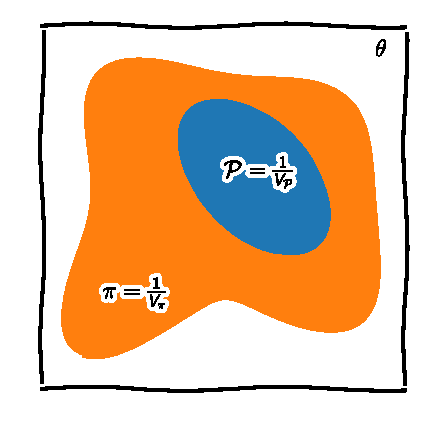
\includegraphics{figures/volumes.pdf}
    \end{columns}
\end{frame}

\end{document}
